\section{Live-Migration-Systeme}
\label{sec:live-migr-syst}
Im Folgenden wollen wir einige konkrete Implementierungen der oben
vorgestellten Techniken vorstellen, und deren Grenzen und
Einsatzbarkeit für die oben genannten Use-Cases betrachten.

\subsection{NomadBIOS und vMotion}
\label{sec:nomadbios--vmware}
Wie im Vortrag von Dr. Jacob Gorm Hansen beschrieben, war die erste
vollständige Implementierung zur Live-Migration einer kompletten \ac{VM}
der NomadBIOS Hypervisor. Asger Jensen und Dr. Jacob Gorm Hansen
entwickelten diesen Hypervisor auf dem L4 Microkernel und
demonstrierten als erste erfolgreich Live-Migration von virtuellen
Maschinen über ein lokales Netzwerk. Die Motivation dieser Arbeit kam
aus dem Grid-Computing: Für jeden Job sollte eine \ac{VM} gestartet werden,
die dann, mit Prioritäten ausgestattet, durch das Grid verschoben
werden konnte, auf der Suche nach freien Ressourcen. Daher rührt auch
der Name \emph{NomadBIOS}, ein "`nomadisches"' System.

Im Rahmen ihrer Master-Arbeit implementierten Jacob Gorm Hansen und
Asger Kahl Henriksen den Hypervisor zunächst auf dem L4
Kernel. Gastsysteme mussten angepasst werden, um auf diesem
teilvirtualisierten System als Userspace Prozess ausgeführt zu
werden. Im Umkehrschluss konnten viele der Prinzipien hinter
Prozessmigration verwendet werden, um Betriebssystemprozesse zu
verschieben. Außerdem verwendet das NomadBIOS \emph{Checkpointing},
den Akt, den Speicherzustand von Prozessen einzufrieren um sie später
fortsetzen zu können.

\subsubsection{Implementierungsdetails des NomadBIOS}
\label{sec:impl-des-nomadb}
Im NomadBIOS werden mehrere Userspace Module für den L4 Kernel
implementiert, die dazu dienen, Gastbetriebssysteme von der Hardware
zu isolieren~\cite{hansen2002nomadic}. Dazu gehören \emph{Paging}, für
die Isolation des Speichermanagements, \emph{Interrupt Multiplexing}
um Zugriff auf Hardware zu verweben und \emph{Address Space
  Translation}, um einfache Kommunikation zwischen dem Gast- und dem
Hostbetriebssystem zu ermöglichen. Letzteres wird genutzt, um
Unterstützung für den Migrationsvorgang im Gastsystem implementieren
zu können.

\begin{figure}[b]
  \centering
  \includegraphics[width=0.7\linewidth]{images/nomad_stage1}
  \caption{NomadBIOS: 1. Migrationsphase}
  \label{fig:nomad_stage1}
\end{figure}
Für die eigentliche Migration implementiert das NomadBIOS ein
\emph{Precopy} Scheme, wie es bereits aus der Prozessmigration bekannt
ist~\cite{hansen2002nomadic}.
\begin{enumerate}
\item In Abbildung~\ref{fig:nomad_stage1} ist der Startzustand der
  Migration dargestellt. Initial ist der Zustand allen Speichers auf
  dem Zielsystem unbekannt (helles Grau). Der gesamte Speicher vom
  Ursprungssystem muss zum Kopieren ausgewählt werden (rot). Der
  Speicher auf dem Ursprung, der dem Gastsystem gehört, wird zunächst
  für Schreibzugriffe gesperrt und der Kopiervorgang auf den neuen
  Host wird gestartet. Wenn währenddessen Speicher geschrieben wird,
  wird ein Page-fault ausgelöst, und das NomadBIOS kann die
  entsprechende Speicherseite erneut zum Kopieren markieren. Danach
  wird die Seite als für das Gastsystem beschreibbar markiert und
  geschrieben.
\item Nach einem ersten Kopierdurchlauf werden so eine Reihe von
  Speicherseiten noch zum Kopieren markiert worden sein. Es ist nicht
  klar ob diese Seiten vor oder nach der letzten Manipulation zum
  Zielsystem kopiert wurden (Abb.~\ref{fig:nomad_stage2}). Diese
  können nun in einem weiteren, kürzeren Kopierdurchlauf mit dem
  Zielsystem synchronisiert werden. Da dieser zweite Kopiervorgang
  schneller vonstatten geht, werden währenddessen weniger Seiten
  wieder vom Gastsystem beschrieben werden.
\item Nach mehreren Iterationen ist das Delta zwischen dem Gast und
  Zielsystem so weit geschrumpft, dass die verbleibende Differenz in
  wenigen Millisekunden kopiert werden kann. In diesem Moment wird der
  Gastprozess auf dem Ursprungssystem eingefroren, die restlichen
  Seiten kopiert, und auf dem Zielsystem gestartet
  (Abb.~\ref{fig:nomad_stage3}). Wenn im gleichen Moment auch das
  Routing angepasst wird, so kann die \ac{VM} direkt weiterarbeiten, ohne
  das Benutzer mehr als einen kurzen Latenzanstieg bemerken.
\end{enumerate}
\begin{figure}[t]
  \centering
  \includegraphics[width=0.7\linewidth]{images/nomad_stage2}
  \caption{NomadBIOS: 2. Migrationsphase}
  \label{fig:nomad_stage2}
\end{figure}
\begin{figure}[b]
  \centering
  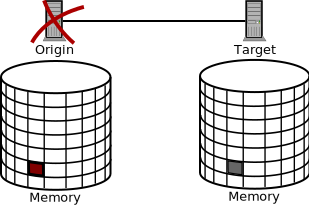
\includegraphics[width=0.7\linewidth]{images/nomad_stage3}
  \caption{NomadBIOS: 3. Migrationsphase}
  \label{fig:nomad_stage3}
\end{figure}

Dr. Hansen arbeitet seit 2007 bei VMWare. VMWare bietet inzwischen ein
kommerzielles Produkt zur Live-Migration names \emph{vMotion}. Der
primäre Fokus dieses Produktes liegt, ähnlich wie beim NomadBIOS,
darin \acp{VM} innerhalb eines Netzwerkes mit gemeinsamem Speicher wandern
zu lassen, um größtmögliche Ressourcennutzung zu erzielen. Dazu bietet
VMWare vMotion die Möglichkeit, sog. \emph{Resource Pools} zu
definieren, in denen \acp{VM} fortwährend automatisiert wandern
können. 

Um höhere Verfügbarkeit zu gewährleisten, weicht vMotion vom oben
etablierten Precopy-Schema ab~\cite{nelson2005fast}. Im letzten
Schritt wird die Ziel-\ac{VM} direkt gestartet, wenn die Ursprungs-\ac{VM}
eingefroren wird. Damit wird vermieden, dass beim Übertragen des
letzten Deltas eventuell offene TCP Verbindungen einen Timeout
erfahren. Die noch zum Kopieren ausstehenden Speicherseiten sind
markiert, und werden noch in die Ziel-\ac{VM} kopiert. Wenn
zwischenzeitlich darauf zugegriffen werden soll, werden sie als
nächstes über das Netzwerk zum Ziel übertragen. Das bedeutet, dass zu
Beginn der Laufzeit der Ziel-\ac{VM} noch eine Abhängigkeit zum
Ursprungssystem besteht, und die Verbindung zwischen beiden Systemen
noch kurze Zeit weiterbestehen muss.

Eine weitere Besonderheit an der VMWare Lösung ist, dass der VMWare
ESX Hypervisor über Para-Virtualisierung hinausgeht, und deshalb die
Migration von beliebigen Betriebsystemen zwischen beliebigen (von
VMWare unterstützten) Hardware Architekturen
unterstützt~\cite{nelson2005fast}. Dafür wird Netzwerkhardware voll
virtualisiert, außerdem wird davon ausgegangen, dass Verbindungen zu
Speicher ausschließlich über \ac{SAN} oder \ac{NAS} bereitgestellt
werden, und dass alle \acp{VM} mit denselben \ac{SAN}-
bzw. \ac{NAS}-Servern verbunden sind.

\subsection{IBM}
IBM unterstützt die Linux Community in großem
Umfang~\cite{kroahhartman2007linux}. IBM hat zur Live-Migration von
Linux-\acp{VM} sowohl beim Xen Projekt, als auch dem Kernel
Virtualisierungsmodul \ac{KVM} im Rahmen des RESERVOIR Projektes
wesentliche Beiträge geleistet~\cite{rochwerger2009reservoir}. Dabei
lag der Fokus der angestrebten Lösung explizit auf Interoperabilität
zwischen verschiedenen Providern und der Möglichkeit, Migration über
Distanzen hinweg zu ermöglichen. Beides zusammen soll die Kosten für
benötigte Infrastruktur (wie z.B. \ac{SAN}-/\ac{NAS}-Server) senken
und die Skalierbarkeit über die Grenzen eines einzelnen Cluster
Netzwerks hinweg erhöhen.

Die Lösung hierfür sind \acp{VEEM}. Ein \ac{VEEM} verteilt \acp{VM}
(in diesem Kontext \acp{VEE} genannt) über verfügbare Host-Systeme,
unter Berücksichtigung bestimmter Einschränkungen, dazu können
z.B. auch gesetzliche Bedingungen oder \acp{SLA} zählen. Außerdem
können mehrere \acp{VEE} zu einer \ac{VEE}-Gruppe zusammengefasst
werden, um bestimmte Dienste nah beieinander zu halten und nur
gemeinsam zu verwalten. IBM hat hierbei speziell darauf geachtet,
offene Protokolle zu erstellen, um die Struktur der Lösung unabhängig
von den verwendeten Virtualisierungsplatformen (\zB Hypervisoren) zu
machen. Auf diese Weise wird ein Migrationspfad für Cloud Anbieter
geöffnet, der es ermöglicht, bestehende Infrastruktur inkrementell mit
den nötigen \acp{API} auszustatten und so interoperabel mit vielen
verschiedenen Cloud-Lösungen zu werden.

\subsection{HP}
HP bietet Virtualisierungsdienste auf Basis von Microsoft's
\emph{HyperV}. \emph{HyperV} unterstützt in Windows Server 2008 R2
bereits Live-Migration von virtuellen Maschinen, der Migrationsprozess
läuft dabei analog zum NomadBIOS ab. Eine wesentliche Limitierung des
HyperV ist, dass alle physikalischen Maschinen Zugriff auf gemeinsamen
Speicher, z.B. Network-Attached-Storage oder ein Netzwerkdateisystem,
haben müssen, um \ac{VM} Daten auszutauschen~\cite{hp2010hyperV}. Das kann
beim Umziehen zwischen geografisch entfernten Orten oft nicht
gewährleistet werden. HP hat hierfür sein \ac{CLX} Produkt
erweitert. \ac{CLX} ist zunächst eine Software zur Replikation von Daten
über große Distanzen. Mit den HyperV spezifischen Erweiterungen kann
\ac{CLX} nun dazu genutzt werden, den Zustand von \acp{VM} zwischen
verschiedenen Rechenzentren zu synchronisieren. Dabei ist \ac{CLX} voll in
den HyperV Live-Migration Prozess integriert. Mit der \ac{CLX}---HyperV
Kombination kann sichergestellt werden, das Replikation über
Datencenter hinweg \ac{VM}-Migrationen unterstützt, und nicht behindert,
indem während der Migration dieser mehr Bandbreite zugestanden wird,
damit die finale Speicherseitensynchronisation (während der die
Ursprungs-\ac{VM} eingefroren ist) so schnell wie möglich vonstatten
geht. Wenn die Migration abgeschlossen ist, macht \ac{CLX} den neuen
physikalischen Standort der \ac{VM} automatisch zum Master für die weitere
Replikation.

Im März 2010 aktualisierte außerdem seine UNIX Distribution
\emph{HP-UX}. Teil dieses Updates war die Version 4.2 des hauseigenen
\emph{Integrity Virtual Machines} Hypervisors. Dieser enthält eine
\emph{Online Migration} Funktion, die ebenso mit \ac{CLX} zusammen
eingesetzt werden kann~\cite{hp2010integrity}.

\subsection{Oracle}

Oracle (vormals Sun) biete in Solaris eine betriebssystemintegrierte
Form der Virtualisierung an: Solaris Zones. Im Gegensatz zu den vorher
vorgestellten Lösungen werden in den Zones keine vollständigen
Betriebsysteme ausgeführt, vielmehr gibt es eine
Betribessysteminstanz, gennant \emph{global zone}, in der der
Betriebssystemkern läuft und mehrere \emph{non-global zones}, die
diesen Kern mitbenutzen. Den \emph{non-global zones} erscheint der
Kern jedoch als ihr "`eigener"'. Solaris Zones werden zumeist zur
Separierung von Applikationen genutzt und mit Resourcenmanagement
verbunden; die Kombination wird \emph{Solaris Container} genannt~\cite{price2004solaris}.

Im Kontext von Live-Migration sind Solaris Zones (und damit auch
Container) jedoch ungeeignet. Es existieren keinerlei Vorrichtungen
dafür im Kern von Solaris, geschweige denn Werkzeuge. Auch
nicht-Live-Migrationen sind mit hohem Manuellen aufwand verbunden und
entsprechen eher dem Prozess "`Herunterfahren, exportieren, kopieren,
importieren, hochfahren"'~\cite{Kimchi:Solaris-Zones-m}. Die Migration
von Zones als Standard-Anwendungsfall ist in Solaris nicht vorgesehen.

Oracle \acfp{ldom} (jetzt VM Server for SPARC), die auf SPARC-Servern
der T-Serie und einigen anderen Systemen zur Verfügung stehen,
unterstützen sein der Version 1.2 aus dem Jahr 2009
Live-Migration~\cite{Laurent:Answering-a-cus}. Diese
hardware-gestützte Virtualisierungsvariante bietet physisch getrennte
Gast-Systeme (Domänen) und dabei die Rekonfigurierbarkeit dieser im
eingeschalteten Zustand. Zur Live-Migration von Domänen wird auf
beiden Seiten nicht nur die selbe Software (in dem Fall auch Firmware)
genutzt, auch die Hardware muss in Prozessortyp und -frequenz
übereinstimmen. Es ist auch nicht möglich, von Vornherein bestimmte
Auslastungsgrenzen zu bestimmen, ab denen eine Live-Migration
vorgenommen wird. Vielmehr wird bei Auslastungsändereungen direkt auf
dem Server reagiert, indem \zB Prozessoren dazu- oder abgeschaltet
werden oder der für die Domäne verfügbarer Speicher verändert
wird~\cite{2010:Oracle-VM-Serve}. Als Betriebssystem in den \acp{ldom}
sind praktisch nur Solaris (und -- dank Linux-Kern-Emulation in
bestimmten Solaris Zones -- ältere Linux) bekannt, theoretisch ist es
aber möglich, beliebige Betriebssystem, die SPARC-Tx-Prozessoren
unterstützen, zu nutzen; so \zB natives Linux~\cite{Chartre:Linux-with-LDom}.



\subsection{Vergleich}
Wir kehren nun zurück zu den zuvor beschriebenen Anwendungsfällen für
\ac{VM}-Live-Migration (\autoref{sec:livemigration}). Die Fähigkeiten und Ziele
der in \autoref{sec:live-migr-syst} beschriebenen Lösungen
machen sie unterschiedlich gut für die beschriebenen Zwecke
einsetzbar (\autoref{tab:anw-anb-matrix}). \emph{Notabene: } Für
Oracle wurde nur die \ac{ldom}-Variante betrachtet.

\onlydraft{
Vergleich der Eignung als Lösung für die oben genannten Probleme
zwischen dem von Dr. Jacob Gorm Hansen vorgestellen System und den Alternativen.
}


\begin{table}[tb] 
  \caption{Anwendung --- Anbieter Matrix}
  \centering
  \begin{tabular}[h]{c|c c c c}
    & VMWare & IBM & HP & Oracle \\
    Verlässlichkeit & & \checked & &  \\
    Interoperabilität & \checked & \checked & &  \\
    Inter-Cloud Verschiebungen & & \checked & & \\
    Hardware Maintenance & \checked & \checked & \checked & \\
    Adaptive Auslastung & \checked & & & (\checked) \\
    Erzwungene Verschiebungen & \checked & \checked & \checked &
    \checked \\
  \end{tabular}
 \label{tab:anw-anb-matrix}
\end{table}


%%% Local Variables: 
%%% mode: latex
%%% TeX-master: "FelgentreffPape_2010_Live-MigrationInVirtuellenUmgebungen"
%%% End: 
